\section{Implementación}

La fase de implementación consistió en llevar a cabo el circuito diseñado. Se montó el prototipo físico utilizando una protoboard para la interconexión de todos los componentes. El Arduino Uno se conectó al módulo de visualización MAX7219, asegurando que las conexiones de datos, reloj y carga se correspondieran con las especificaciones del diseño. Los dos botones pulsadores se integraron al circuito para permitir la interacción, configurados para incrementar y decrementar el valor del contador. El código desarrollado se cargó en el microcontrolador, permitiendo la correcta operación del sistema según la lógica de control definida. El resultado de este proceso de montaje es el prototipo funcional que se ilustra a continuación:

\begin{figure}[H]
\centering
 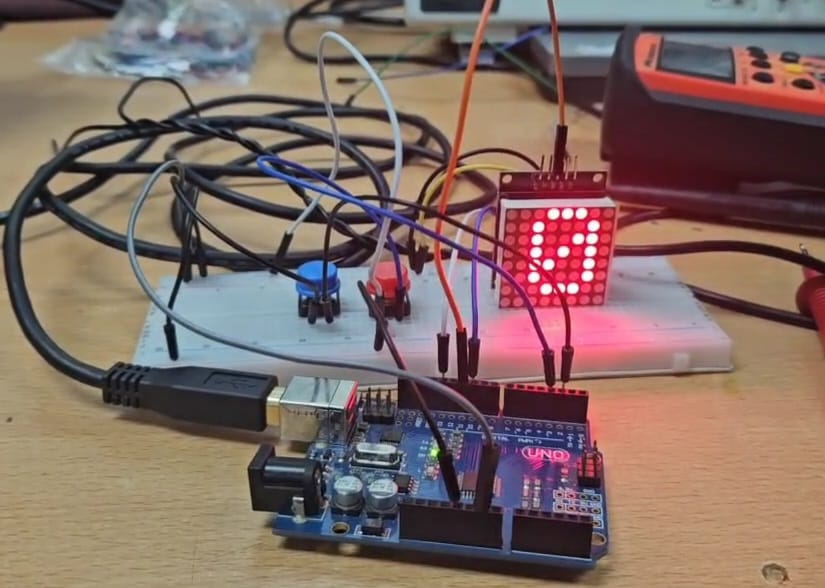
\includegraphics[width=0.8\textwidth]{Diagramas/implemen.jpg}
\caption{Implementación del prototipo en el laboratorio.}
\label{fig:implementacion_laboratorio}
\end{figure}
